
\chapter{\IfLanguageName{dutch}{Praktische uitvoering van ANPR}{Implementation of ANPR at UGent}}
\label{ch:praktischeUitvoering}
In dit hoofdstuk zal er onderzocht worden of nummerplaatdetectie degelijke resultaten kan leveren op de Campus Sterre en Campus Coupure van UGent. Hiervoor zullen handmatig foto's genomen worden van wagens die de parking willen verlaten met de Pi-NoIR cam. Hierna wordt er gecontroleerd of OpenANPR wel degelijk correcte resultaten levert op de genomen foto's.


\section{Hardware en software}
In dit onderdeel wordt de opstelling en configuratie van de camera's uitgelegd adhv. de informatie verzameld in Hoofdstuk \ref{ch:maatregelenanpr}.

\subsection{Camera}
Als camera zal gebruik gemaakt worden van de PiNoIR-Cam. Deze camera is een standaard extensie voor de Raspberry-PI die geen infrarood filtering heeft staan. Standaard wordt infrarood uit afbeeldingen gefilterd omdat deze een ongewenst bijproduct zijn op foto's. De PiNoIR camera filtert geen infrarood uit de afbeeldingen en maken het dus mogelijk om te gebruiken voor infrarood detectie.

\paragraph{Cameraplaatsing}
Voor de plaatsing van de camera's wordt er gewenst zo veel mogelijk kosten te besparen en wordt er liever niet geopteerd voor een aparte paal voor de ANPR-camera. Daarom zal als fotopunt de metalen constructie van de hefboom gekozen worden. De camera zal hier op de top worden aangehangen zodat deze zo min mogelijk interferentie heeft van de koplampen van de auto's.

\begin{figure}[h!]
	\centering
	\includegraphics[width=\linewidth]{img/uitgang-coupure.jpg}
	\caption{Uitgang met tokens aan UGent campus Coupure}
\end{figure}

\paragraph{Cameraconfiguratie}
De voorgaande camerainstellingen zullen zo correct mogelijk op de PiNoIR camera worden ingesteld.
TODO: configuratie bepalen



\subsection{Opstelling}
Om de foto's te verkrijgen zal gebruik gemaakt worden van de Raspberry Pi met de PiNoIR camera, deze zal in een behuizing op de juiste hoogte van de paal tijdelijk vastgezet worden tesamen met een powerbank. Om het signaal te sturen dat de Raspberry Pi een foto moet nemen zal deze ingesteld worden als Access Point, zo kan er via een GSM een SSH verbinding gemaakt worden waarop men de camera bestuurt.

Figuur \ref{Opstelling} toont de gemaakte opstelling. Deze bevat De Raspberry Pi, de Pi-Cam en een powerbank met een capaciteit van 700mAh.
\begin{figure}[h]
	\centering
	\includegraphics[width=0.5\linewidth]{img/camera.jpg}
	\caption{Opstelling Raspberry Pi met PiCam.}
	\label{Opstelling}
\end{figure}

\section{Verzamelen van de gegevens}

Om een correcte dataset te bekomen zal er op de parking van UGent zelf data verzameld worden aan de uitgangen.
Deze uitgangen zijn:
\begin{itemize}
	\item Campus Coupure - Uitgang Coupure Links
	\item Campus Coupure - Uitgang Kruisboogstraat
	\item Campus Landbouw - Uitgang De Pintelaan
	\item Campus Landbouw - Uitgang Galglaan
\end{itemize}

Hierbij worden er 2 tot 3 foto's genomen per auto.
Aan al deze uitgangen zijn er in totaal 252 foto's genomen op volgende momenten:

Motion detection:


\begin{table}[h]
\centering
\begin{tabular}{l|l|l|l|l}
	Datum 		& Begin & Eind	& Locatie	& Aantal foto's \\ \hline
	06/11/2019	& 11u45 & 12u46	& Campus Coupure - Uitgang Kruisboogstraat	& 53	\\
	08/11/2019	& 12u15 & 12u29	& Campus Sterre - Uitgang Galglaan	& 22	\\
	08/11/2019	& 12u52 & 13u41	& Campus Sterre - Uitgang De Pintelaan	& 38	\\
	13/11/2019	& 11u36 & 12u08	& Campus Sterre - Uitgang De Pintelaan	& 50	\\
	13/11/2019	& 12u29 & 12u42	& Campus Sterre - Uitgang Galglaan	& 10	\\
	13/11/2019	& 13u48 & 14u35	& Campus Coupure - Uitgang Coupure Links	& 5	\\
	14/11/2019	& 18u05 & 18u55	& Campus Coupure - Uitgang Coupure Links	& 3	\\
	21/11/2019	& 14u08 & 15u11	& Campus Sterre - Uitgang De Pintelaan	& 35	\\
	21/11/2019	& 15u58 & 16u22	& Campus Sterre - Uitgang Galglaan	& 36	\\
\end{tabular}
\end{table}

Zo bekomen we volgende aantallen van foto's per uitgang:
\begin{table}[h]
	\centering
	\begin{tabular}{l|l}
		Uitgang	& Aantal foto's \\ \hline
		Campus Coupure - Uitgang Kruisboogstraat	& 53\\
		Campus Coupure - Uigang Coupure Links	& 5\\
		Campus Sterre - Uitgang Galglaan	& 32\\
		Campus Sterre - Uitgang De Pintelaan, camerahoek rechts	& 38\\
		Campus Sterre - Uitgang De Pintelaan, camerahoek links	& 50\\
	\end{tabular}
\end{table}

Per nummerplaat wordt volgende data genoteerd:
\begin{itemize}
	\item \textbf{file:} De bestandsnaam van de foto.
	\item \textbf{license\_plate:} De 'correcte' nummerplaat, handmatig uit de foto gehaald.
	\item \textbf{result:} De nummerplaat gedetecteerd door OpenALPR.
	\item \textbf{correct:} Een booleaanse waarde of de nummerplaat overeenkomt.
	\item \textbf{distance:} De afstand van de camera, bestaat uit 3 velden, "close", "medium"\ en "far". Close betekent een afstand onder de 3 meter, medium tussen 3 en 5 meter en far betekent verder dan 5 meter.
	\item \textbf{lighting:} De belichting van de nummerplaten, bestaat uit 2 velden, "bright"\ en "very\_bright". Bright betekent dat de nummerplaat duidelijk leesbaar is voor mensen onder normaal daglicht. very\_bright betekent dat deze niet onmiddelijk leesbaar is.
	\item \textbf{location:} De uitgang waar de foto is genomen, bestaat uit "coupure-kruisboogstraat", "coupure-coupurelinks", "sterre-galglaan"\ en "sterre-depintelaan".
\end{itemize}

\section{Verwerking van gegevens}

Na de foto's gemaakt zijn worden deze geclassificeerd volgens nummerplaat, belichting, locatie en afstand van de camera. Vervolgens wordt er nummerplaatdetectie uitgevoerd met behulp van OpenALPR en worden worden deze bij de bij de foto opgeslaan.

Per auto worden 2-3 foto's bijgehouden, deze worden geselecteerd op basis van de afstand. De auto dient op minstens 2 verschillende afstanden gedetecteert te zijn, dit om te voorkomen dat foto's van onrepresentabele afstanden genomen zijn. Het nemen van de foto's is via een handmatige trigger en heeft dus de mogelijkheid dat de foto's niet op een representabele afstand zijn. In een echte implementatie wordt er een automatische triggering van de camera's gebruikt.23

De detectie van een nummerplaat is succesvol indien één van de genomen foto's correct is.
twee afstanden per auto.

\subsection{Calibratie van de afbeeldingen}
Origineel waren de resultaten van de nummerplaatdetectie aan de zeer lage kant, aangezien de afbeeldingen nog niet gekalibreerd waren. OpenALPR een horizontale nummerplaat in de afbeeldingen, wat niet mogelijk te bereiken  is puur met de Pi-Cam.
\begin{figure}[h!]
	\centering
	\begin{subfigure}[b]{0.4\linewidth}
		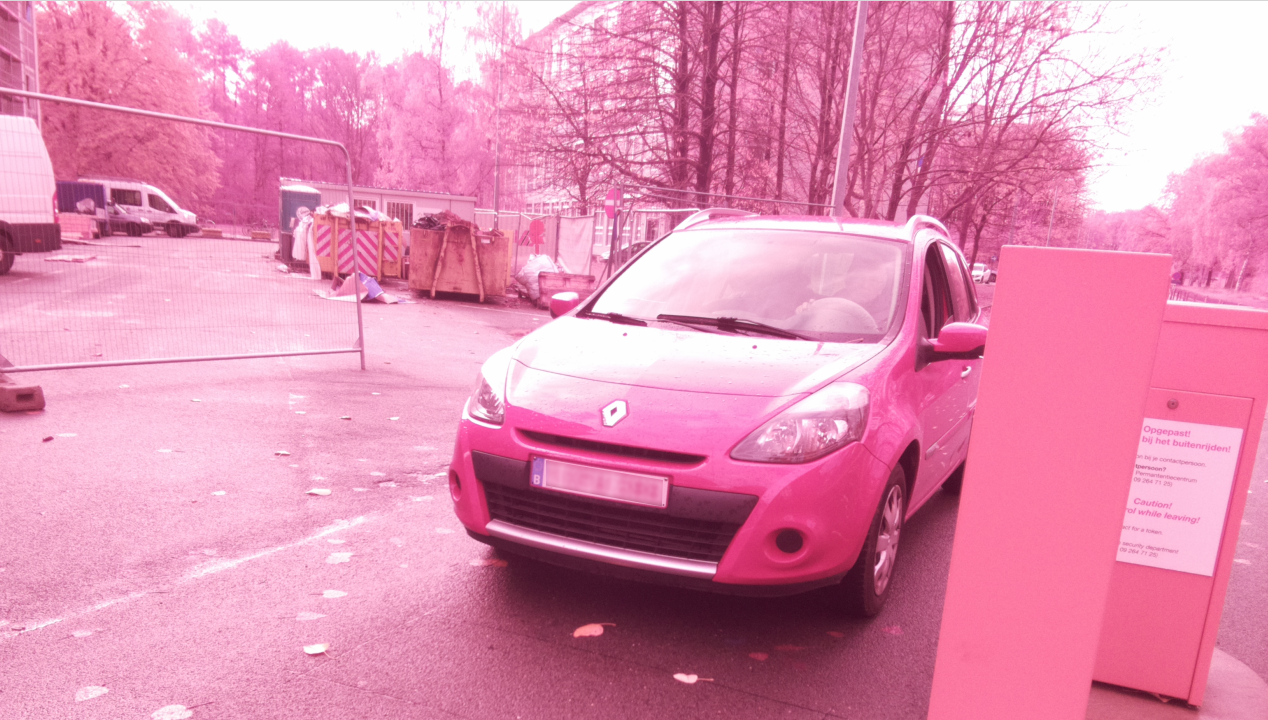
\includegraphics[width=\linewidth]{img/calibration/pre-calibrate.png}
		\caption{Niet-gekalibreerde afbeelding}
	\end{subfigure}
	\begin{subfigure}[b]{0.4\linewidth}
		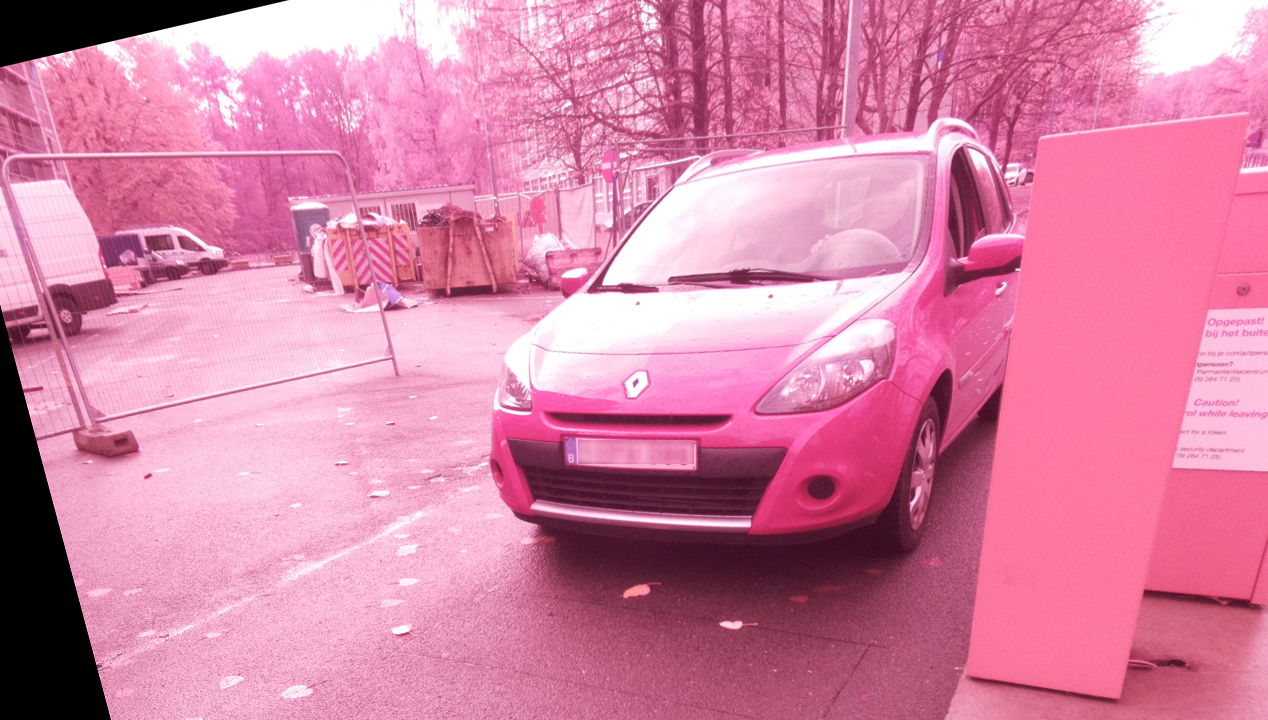
\includegraphics[width=\linewidth]{img/calibration/calibrate-cut.png}
		\caption{Gekalibreerde afbeelding}
	\end{subfigure}
	\label{fig:calibration}
	\caption{Calibratie van afbeeldingen met behulp van openalpr-utils-calibrate.}
\end{figure}

Een verduidelijking van het het verschil van de resultaten aan de uitgang van Campus Sterre - Galglaan:
\begin{table}[h]
	\centering
	\begin{tabular}{l|l|l|l}
		 		& Incorrect & Correct & Ratio	\\ \hline
		Niet-gekalibreerd	& 25 & 2 & 7.4\%	\\
		Gekalibreerd	& 9 & 18 & 66.7\%\\
	\end{tabular}
\end{table}

\section{Resultaten}

\subsection{Campus Sterre - Uitgang Galglaan}

\begin{table}[h]
	\centering
	\begin{tabular}{l|l|l|l|l}
\textbf{Campus Sterre uitgang galglaan} & Totaal & Incorrect & Correct & Ratio	\\ \hline
Per individuele foto 	& 62 & 21	& 41	& 66.13\%\\
Per auto				& 24 & 3	& 21 	& 87.5\%\\
\end{tabular}
\end{table}



Eind subsectie galglaan

De eerste resultaten aan de uitgang van (coupure1) waren niet veelbelovend, dit kwam doordat in de gekozen orientatie er 's ochtends interferentie was van het zonlicht, de gekozen locatie van de camera is dus geen correcte keuze. Dit is te zien op Afbeelding \ref{SterreZonlicht}. Deze afbeelding is niet bewerkt, de nummerplaat is helemaal niet zichtbaar door de reflectie van het zonlicht.
\begin{figure}[h!]
	\centering
	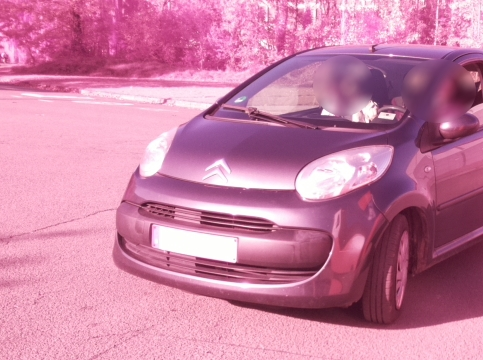
\includegraphics[width=0.5\linewidth]{img/sterre2zon.jpg}
	\caption{Interferentie van zonlicht op de parking van Campus Sterre.}
	\label{SterreZonlicht}
\end{figure}

In het donker is de interferentie van de koplampen niet te groot, maar de algemene donkerheid van de omgeving zorgt ervoor dat de raspberry pi zijn shutter te lang openhoudt en dat de afbeeldingen enorm donker blijken. Het is dus vereist om extra infraroodbelichting bij te plaatsen.
\begin{figure}[h!]
	\centering
	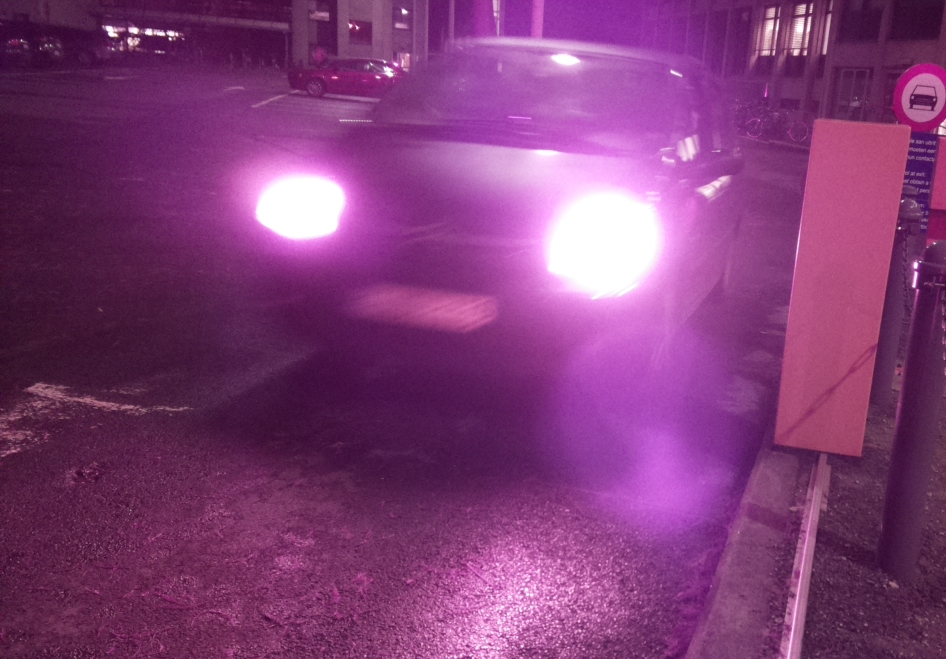
\includegraphics[width=0.5\linewidth]{img/nacht-coupure.jpg}
	\caption{Interferentie van zonlicht op de parking van Campus Sterre.}
	\label{SterreZonlicht}
\end{figure}

Resultaten overdag, per afbeelding
\begin{table}[h]
	\centering
	\begin{tabular}{l|l|l|l|l}
		Uitgang	& Aantal foto's & Incorrect	& Correct & Ratio \\ \hline
		Campus Coupure - Uitgang Kruisboogstraat &	52	& 15	& 37	&	71.2\% \\
		Campus Coupure - Uitgang Coupure Links	& / & & \\
		Campus Sterre - Uitgang Galglaan &	62	& 21	& 41 & 66.13\%\\
		Campus Sterre - Uitgang De Pintelaan	& 73	& 47	&	26	& 35.6\%\\ \hline
		Totaal & 188 & 83 & 105 & 44.1\%
	\end{tabular}
\end{table}

Resultaten overdag, per auto
\begin{table}[h]
	\centering
	\begin{tabular}{l|l|l|l|l}
		Uitgang	& Aantal auto's & Incorrect	& Correct & Ratio \\ \hline
		Campus Coupure - Uitgang Kruisboogstraat& 23 & 2	& 21 	& 91.3\% \\
		Campus Coupure - Uitgang Coupure Links	& / & &   	& 	\\
		Campus Sterre - Uitgang Galglaan		& 24 & 3	& 21 	& 87.5\%\\
		Campus Sterre - Uitgang De Pintelaan	& 25 & 10	& 15		& 60.0\%\\ \hline
		Totaal & 72 & 15 & 57 & 79.2\%
	\end{tabular}
\end{table}


\section{Conclusie}

\section{Uitbreidingen}
Locatie van de sensor kan mss in het midden van balk \autocite{buhus2016automatic}.